\documentclass[a4paper,11pt,titlepage]{article}
 
\usepackage[utf8]{inputenc}
\usepackage[spanish]{babel}
\usepackage[T1]{fontenc}
\usepackage{lmodern}
 
\usepackage{parskip}
\usepackage{graphicx}
\usepackage{xcolor}
 
\definecolor{gris}{RGB}{220,220,220}
 
\begin{document}
\begin{titlepage}
  \vspace*{1cm}
  {\fontsize{15}{34}\selectfont\bfseries Universidad Politecnica Zona Metropolitana De Guadalajara} \\\\
  {\large Titulo Del Proyecto: Sistemas De Riego Automatico }\\\\
  {\large segundo Avance} \\\\
  {\large ingenieria mecatronica} \\\\
  \large {Profesor: Moran Garabito Carlos Enrique} \\\\
  {\large Integrantes:} \\
  {\large Hernandez Cardenas Oscar Osvaldo} \\\
  {\large Banda Macías Francisco Javier} \\\
  {\large Cedano Gutiérrez Nancy Noemí} \\\
  {\large Sánchez López Irad Yabhel} \\\
  {\large 4 A} \\\
   
  \hfill
  % Logo
  
\includegraphics[height=8cm]{upzmg.jpeg} \\
  % Línea gris
  {\color{gris}\hrule}
 
  \vfill
   {\hfill 18-Oct-19} \\
   
\section{Planteamiento del problema}
En la universidad politécnica de la zona metropolitana de Guadalajara tienen bastante terreno
verde, hace unos cuatrimestres pasados, se abrió una convocatoria de reforestación en la
universidad. Afortunadamente vimos que muchos fueron los interesados en realizar dicha
actividad y se inició el proceso. Al cabo de unas semanas nos percatamos que el mantenimiento
hacia los árboles plantados no se realizaba como debería ser.
Entonces nos preguntamos ¿Realmente hay un interés por parte de los alumnos el cuidar el medio
ambiente? Y concluimos que realmente los alumnos lo hicieron por simple calificación. Los arboles
estaban secos y nadie se hace cargo de ellos, hay un mal control para cuidar las áreas verdes, si
acaso solo se mantienen en buen estado las de fácil acceso o común acceso. No hay personal
destinado a ello. Para evitar continuar con esta problemática, diseñamos la implementación de un
sistema de riego automático que pueden cubrir
parcialmente toda la universidad e incluso poder implementarlo fuera de ella, esto afectando no
solo a árboles, sino que también a cosechas de consumo grande o masivo.

\section{Objetivo general del proyecto (¿A dónde queremos ir?):}
Desarrollar un proyecto automatizado en el que se cree un sistema de riego automático,
controlado desde una aplicación, con implementación de controladores programables,
investigación acorde a las propiedades de los materiales a utilizar y sistemas electrónicos.

\section{Justificación}
La implementación para estos sistemas de riego no solo es para mantener áreas verdes y que se
vea bonito, esto es para fomentar una cultura para proteger nuestro ecosistema y cultivos,
ofreciendo la posibilidad de regar áreas de difícil acceso, mediante sistemas novedosos como lo es
recibir notificación o recordatorio para dar la indicación desde una app móvil de encender o
apagar el sistema de riego.

\section{Delimitación}
•Escases de recursos económicos para la compra de los materiales.

•El sistema de riego no es tan útil en temporadas de lluvia.

\section{Matriz de posibles materiales y costos}

\begin{tabular}{|c|c|c|}
\hline 
Nombre del Material & • & • \\ 
\hline 
Baquelita & 1 & 50 \\ 
\hline 
Arduino nano & 1 & 240 \\ 
\hline 
I2C Interfaz
 & 1 & 35 \\ 
\hline 
LCD 16*2 & 1 & 79 \\ 
\hline 
Sensor de humedad y temperatura DHT11 & 1 & 59 \\ 
\hline 
Bluetooth HC06 & 1 & 220 \\ 
\hline 
Fotorresistencia LDR  & 1 & 9 \\ 
\hline 
Teclado 4*4 & 1 & 45 \\ 
\hline 
Modulo RTC (Reloj tiempo real) & 1 & 49 \\ 
\hline 
Sensor de humedad suelo & 1 & 40 \\ 
\hline 
Relevadores 5V & 1 & 25 \\ 
\hline 
Bornera 3 pts & 1 & 20 \\ 
\hline 
Diodo 1N4004 & 1 & 8 \\ 
\hline 
Transistor 2N2222A & 2 & 35 \\ 
\hline 
Resistencia 1K & 2 & 2 \\ 
\hline 
Resistencia 10K & 1 & 2 \\ 
\hline 
Resistencia 100k & 1 & 2 \\ 
\hline 
Pin jumper & 3 & 30 \\ 
\hline 
Regleta hembra 40 pin & 3 & 5 \\ 
\hline 
Regleta macho 4 pin & 1 & 5 \\ 
\hline 
Cable H-M & 5 & 24 \\ 
\hline 
\end{tabular} 
                                                                                                      
\section{Explicación de la aportación de cada materia cursada en el cuatrimestre al proyecto}

 % Logo
  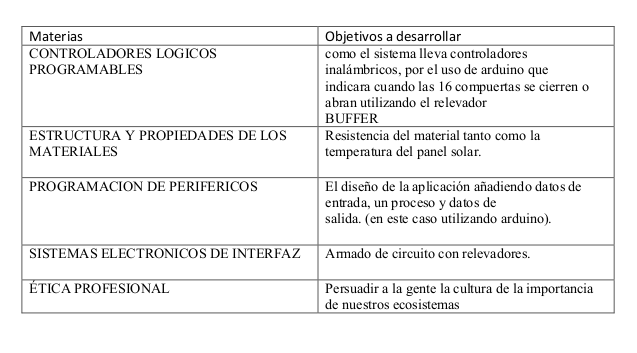
\includegraphics[height=9cm]{cul.png} \\

\section{Boceto del proyecto}


 % Logo
  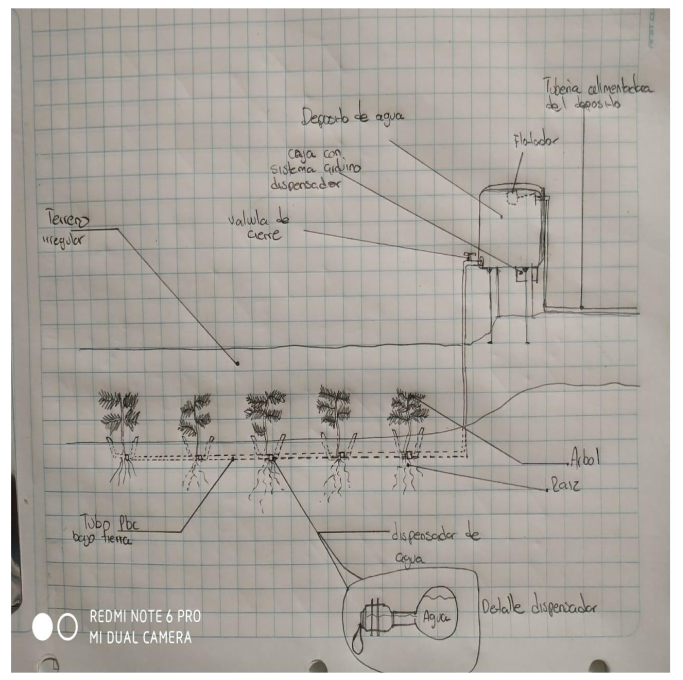
\includegraphics[height=15cm]{boce.png} \\
  
  % Logo
  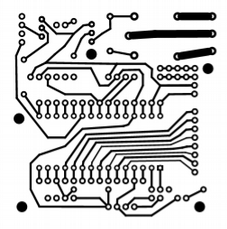
\includegraphics[height=10cm]{imag.png} \\
  
  % Logo
  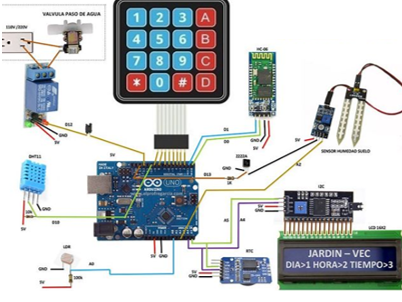
\includegraphics[height=10cm]{teclado.png} \\
                                                                                                                                                                                                                                                                                                                                                                                                        
   
\end{titlepage}
\end{document}
